\documentclass[a4paper]{article}
\usepackage{enumerate}
\usepackage{amsmath}
\usepackage[english]{babel}
\usepackage{url}
\usepackage{graphicx}

\title{k-Nearest-Neighbours\\\large Lab Session 1\\Machine Learning: Pattern Recognition\\Master Artificial Intelligence}

\author{Camiel Verschoor \\StudentID: 10017321\\UvAnetID: 6229298\\ \url{Verschoor@uva.nl} \and Steven Laan\\StudentID: 6036031\\UvAnetID: 6036031\\\url{S.Laan@uva.nl}}

\begin{document}

\maketitle

\section{Data Visualization}
\begin{figure}[!ht]
\centering
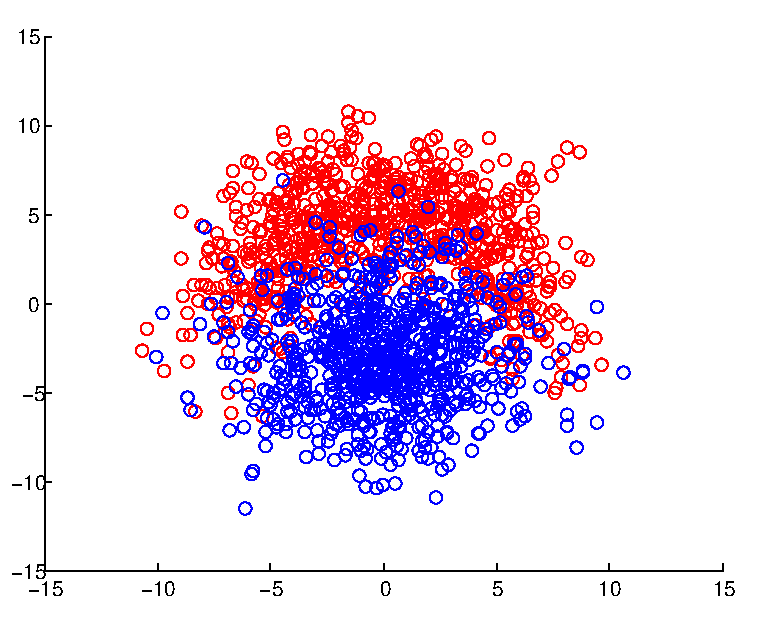
\includegraphics[width=0.75\textwidth]{images/data_scatterplot.pdf}
\caption{Data visualization.}
\label{data}
\end{figure}
In figure \ref{data} the data of the training set is visualized, which consists of the two classes: A (red) and B (blue).

\newpage
\section{k-Nearest Neighbours}
In this lab assignment, a kNN classifier, with $k = 1$, is trained on the trainings data. The performance is evaluated on the test data. This resulted in the following confusion matrix:
\begin{center}
\begin{tabular}{ | l | l | l | }
\hline
 & \textbf{True} & \textbf{False}\\
\hline
\textbf{Positive} & 206 & 44\\
\hline
\textbf{Negative} & 36 & 214\\
\hline
\end{tabular}
\end{center}
From the confusion matrix the error rate is computed by the complement of the accuracy, presented in the following formula:
\begin{equation}
\textit{Error} = 1 - \textit{accuracy} = 1 - \frac{\textit{tp} + \textit{fp}}{\textit{tp} + \textit{tn} + \textit{fp} + \textit{fn}}
\end{equation}
The error rate and other statistical measures of the classifier are presented in the table below:
\begin{center}
\begin{tabular}{ | l | l | }
\hline
\textbf{Accuracy} & 84.0\%\\
\hline
\textbf{Precision} & 82.4\%\\
\hline
\textbf{Recall} & 85.1\%\\
\hline
\textbf{F-measure} & 83.7\%\\
\hline
\textbf{Error rate} & 16.0\%\\
\hline
\end{tabular}
\end{center}
In figure \ref{error_rate}, a graph is shown of the test error evolving as a function of k. Notice that test error increases when $k$ is growing, this is caused by overfitting on the training set. Furthermore, it can be noticed that the function is fluctuating, which is caused by the noise of the classifier.
\begin{figure}[!ht]
\centering
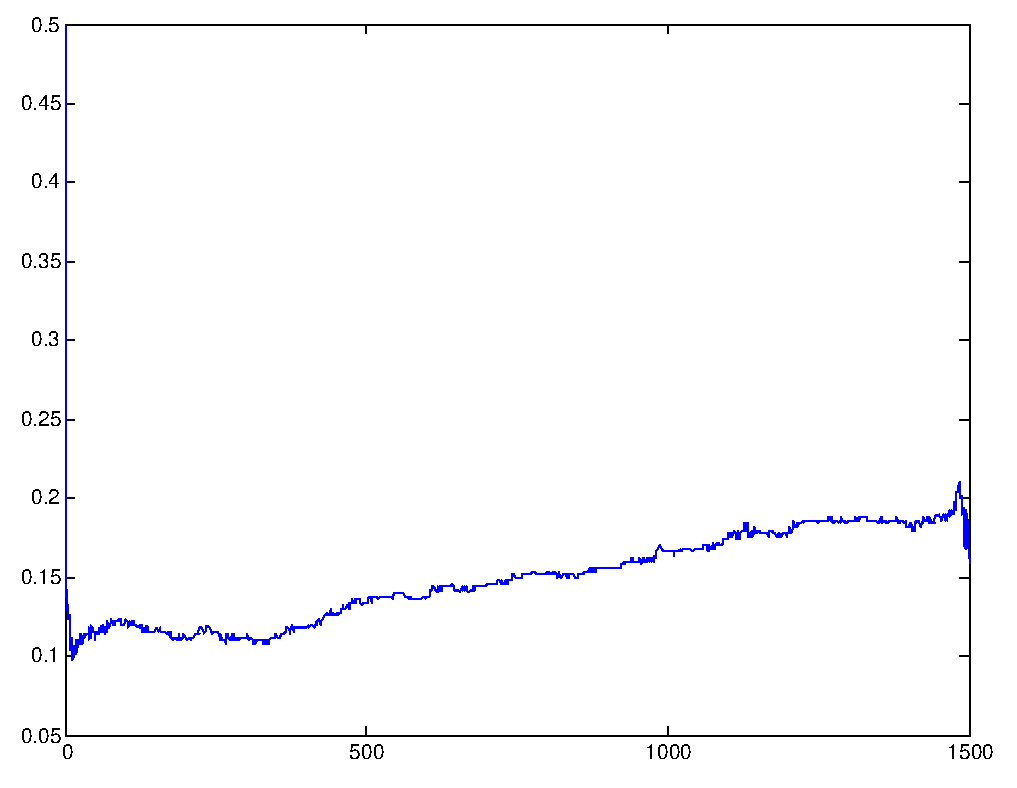
\includegraphics[width=0.75\textwidth]{images/error_rate_1500_1.pdf}
\caption{Graph of the error rate with various $k$}
\label{error_rate}
\end{figure}\\
From this single experiment we \textbf{cannot extract a specific value of $k$}, because it could be the case that the data used for training \textbf{is not representative of the total distribution.} 
If we must decide on a value for $k$, given these results, we would choose something between 100 and 250, because in the graph there is clearly a low plateau. In order to determine which value in the range 100-250, statistical measures like the \textbf{P-test} can be employed. This way we can check statistically which values lie on this minimal plateau. Then we will want to choose the highest value for $k$ that statistically still lies on that plateau. This way we \textbf{generalize the most}, while \textbf{keeping the best performance}. By looking at the graph, we guess this $k$ is 240.

\section{Cross Validation}
The advantage of using evaluation methods like cross-validation and bootstrapping, is that these methods evaluate \textbf{how well} a hypothesis of \textbf{the classifier performs on predicting new data.} Both bootstrapping and cross-validation \textbf{prevent overfitting} caused by a poorly distributed training set. By taking the average hypothesis over a variety of training sets.
Moreover, by using such methods, a better idea of the performance of the model on the real distribution can be obtained.

For this lab assignment, 10-fold cross validation was implemented. For each fold, different values for $k$ were tested. The problem is, as partly explained in the previous section, that \textbf{$k$ with the minimal error is not always the best value for $k$ for the general problem.} This is due to overfitting of the dataset used to train the classifier; the model does not generalize. Therefore, the suggestion was made to take the maximal value of the minimal plateau. However, this method was not implemented, instead the minimal error was taken. Thus, for each fold a range of values of $k$ were tested and the value with the smallest error was kept.

After 10 folds, a list is obtained containing ten values for k. \textbf{The mean of this list is the best guess for $k$ at the moment.} Here we assume that error function does not have weird fluctuations in the center, i.e. when taking the mean we do not end up on a hill, yielding a worse performance than when stuck with one of the values. The result is presented in the following table:
\begin{center}
\begin{tabular}{ | l | l | }
\hline
\textbf{Fold} & \textbf{Best $k$}\\
\hline
1 & 42\\
\hline
2 &347\\
\hline
3 & 75\\
\hline
4 & 145\\
\hline
5 & 11\\
\hline
6 & 4\\
\hline
7 & 5\\
\hline
8 & 723\\
\hline
9 & 159\\
\hline
10 & 3\\
\hline
\textbf{Mean} & 151.4\\
\hline
\textbf{Standard deviation} & 227.9826\\
\hline
\end{tabular}
\end{center}
The above results show that the data in the dataset is scattered, which means that the resulting mean value of k is not very reliable.

Thus if its assumed that the real error function is smooth and does not have weird fluctuations, \textbf{the mean value for $k$ can be used.} The expected form of the error function is a convex shape: at first the classifier under fits the model, thereafter the classifier decreases and reaches its optimal value and finally the function slowly increases as the classifier over fits the model.

Cross-validation is useful, because when employed \textbf{all the training data can be used} to actually train the model. Whereas in the conventional way, you have to keep a part of the training data apart, to evaluate your model. Moreover, cross-validation \textbf{counteracts overfitting.} By leaving parts of the training data out, the model tries to fit itself to less data, which increases the probability of overfitting. However, because the model is averaged over multiple training sessions (on different training sets), this effect will disappear.

The test error is computed by the complement of the accuracy presented in section 2, which is $Error = 1 - accuracy$. This is an estimate of the inaccuracy of the statistical model.

A validation set is a portion of the dataset used \textbf{to asses the performance of prediction or classification models} that have been fit on a separate set, training data, of the dataset. The validation set is used as a \textbf{more objective measure} of performance of various models that have been fit on the training data as validating the performance with the training set is not likely to be a good guide to the performance of the models on new data. 
\end{document}